\RequirePackage{luatex85}
\PassOptionsToPackage{unicode}{hyperref}
\PassOptionsToPackage{naturalnames}{hyperref}
\documentclass{article}
\usepackage{geometry}
\usepackage{fullpage}
\usepackage{parskip}
\usepackage{physics}
\usepackage{amsmath}
\usepackage{amssymb}
\usepackage{xcolor}
\usepackage[colorlinks,linkcolor=blue,citecolor=green]{hyperref}
\usepackage{array}
\usepackage{longtable}
\usepackage{multirow}
\usepackage{comment}
\usepackage{graphicx}
\usepackage{cite}
\usepackage{amsfonts}
\usepackage{bm}
\usepackage{slashed}
\usepackage{dsfont}
\usepackage{mathtools}
\usepackage[compat=1.1.0]{tikz-feynman}
\usepackage{pgfplots}
\pgfplotsset{compat=newest}
\usepackage{simpler-wick} 
\usepackage{mathrsfs}
\usepackage{xparse}
\usepackage{enumerate}
\usepackage{extarrows}
\usepackage{subcaption}

% ==============================================================================
% Minted
% ==============================================================================
\usepackage{minted}
\usemintedstyle{colorful}

% ==============================================================================
% Changes: comments and highlights
% ==============================================================================
\let\comment\undefined
\usepackage[highlightmarkup=uwave]{changes}

\allowdisplaybreaks

% ==============================================================================
% mathtools
% ==============================================================================
\newcommand\MTkillspecial[1]{% helper macro
	\bgroup
	\catcode`\&=9
	\let\\\relax%
	\scantokens{#1}%
	\egroup
	}
\DeclarePairedDelimiter\BraceM\{\}
\reDeclarePairedDelimiterInnerWrapper\BraceM{star}{
	\mathopen{#1\vphantom{\MTkillspecial{#2}}\kern-\nulldelimiterspace\right.}
	#2
	\mathclose{\left.\kern-\nulldelimiterspace\vphantom{\MTkillspecial{#2}}#3}
	}
\let\Bqty\relax
\newcommand{\Bqty}[1]{\BraceM*{#1}}
\DeclarePairedDelimiter\ceil{\lceil}{\rceil}
\DeclarePairedDelimiter\floor{\lfloor}{\rfloor}

% ==============================================================================
% ifthen for User-definition
% ==============================================================================
\usepackage{ifthen}
% HOWTO:
% \ifthenelse{<test>}{<code for true>}{<code for false>}

% ==============================================================================
% User Definition
% ==============================================================================
\newcommand{\red}[1]{{\color{red}#1}}
\newcommand{\mm}[1]{\frac{\dd^4#1}{(2\pi)^4}}
\newcommand{\mme}[1]{\frac{\dd^3\vb{#1}}{(2\pi)^3}}
\newcommand{\mmd}[2][d]{\ifthenelse{\equal{#1}{1}}{\frac{\dd {#2}}{2\pi}}{\frac{\dd^{#1}{#2}}{(2\pi)^{#1}}}}

\makeatletter
\newcommand{\pushright}[1]{\ifmeasuring@#1\else\omit\hfill$\displaystyle#1$\fi\ignorespaces}
\newcommand{\pushleft}[1]{\ifmeasuring@#1\else\omit$\displaystyle#1$\hfill\fi\ignorespaces}
\makeatother

% ==============================================================================
% Tikz-Feynman Externalization
% ==============================================================================
\usepackage{shellesc}
\usetikzlibrary{external}
% \usepgfplotslibrary{external}
\tikzexternalize[shell escape=-enable-write18,prefix=./,system call={lualatex \tikzexternalcheckshellescape -halt-on-error -interaction=batchmode -jobname "\image" "\texsource"},up to date check=diff]

\tikzfeynmanset{
	Eikonal/.style={
		/tikz/draw=none,
		/tikz/decoration={name=none},
		/tikz/postaction={
			/tikz/draw,
			/tikz/double distance=2pt,
			% /tikzfeynman/with arrow=0.5,
		},
	}
}


\title{One Loop Matching for Quasi PDF}
\author{Yingsheng Huang}
\begin{document}
\maketitle
\section{Background}
The definition of parton distribution function (PDF) is 
\begin{align}
	q\left(x, \mu_{f}\right)=\frac{1}{2} \int \frac{d \eta^{-}}{2 \pi} e^{-i x P^{+} \eta^{-}}\left\langle P, S\left|\bar{\psi}\left(0,\eta^{-},\vb{0}_{T}\right) \Gamma \mathcal{W}\left[\eta^{-} ; 0\right] \psi(0)\right| P, S\right\rangle
\end{align}
where with this unpolarized PDF case, $\Gamma=\gamma^+$. $\mathcal{W}$ is the gauge link defined as\cite{Collins2009}
\begin{align}
	\mathcal{W}\left[w^{-}, 0\right]=P\left\{e^{-i g_{0} \int_{0}^{w^{-}} \mathrm{d} y^{-} A_{(0) \sigma}^{+}\left(0, y^{-}, \boldsymbol{0}_{\mathrm{T}}\right) t_{\sigma}}\right\}
\end{align}
The definition of quasi PDF is 
\begin{align}
	\tilde{q}(x)=\frac{1}{2} \int \frac{\dd z}{2 \pi} e^{i x P^{z} z}\langle P, S|\bar{\psi}(z) \tilde{\Gamma} \tilde{\mathcal{W}}[z, 0] \psi(0)| P, S\rangle
\end{align}
where 
\begin{align}
	\tilde{\mathcal{W}}\left[z, 0\right]=\exp \left[i g \mathcal{P} \int_{0}^{z} \dd z^{\prime} n \cdot A^{a}\left(z^{\prime}\right) \mathrm{t}^{a}\right], n^\mu=(0,0,0,-1)
\end{align}
and $\tilde{\Gamma}=\gamma^z$ in our case. 

To make the gauge links equal to unity, we choose light cone gauge for PDF and axial gauge for quasi PDF. 

\section{Tree Level Matching}
In axial gauge, the quasi PDF is
\begin{align}
	\tilde{q}(x)=\frac{1}{4 \pi} \int \dd z e^{i x P^{z} z}\langle P|\bar{\psi}(z) \gamma^{z}\psi(0)| P\rangle
	\label{quasipdf}
\end{align}
The frame is chosen such that $P^{\mu}=(P^0,\vb{0},P^z)$. 
\begin{align}
	P^0=\sqrt{m^2+{P^z}^2}
\end{align}
Up to one loop, we can use quark state as the external state to complete the matching process. The quark field $\psi$ reads
\begin{align}
	\psi(x)=\int \frac{\dd^{3} \vec{k}}{(2 \pi)^{3}} \frac{1}{2 E_{k}}\left[u(k) e^{-i k \cdot x} b_{k}+v(k)e^{ik\cdot x} d_{k}^{\dagger}\right]
\end{align}
Insert it to \eqref{quasipdf}
\begin{align}
	\tilde{q}^{(0)}(x)&=\int \frac{\dd z}{4 \pi}  e^{i x P^{z} z}\mel{0}{b_P \int \frac{\dd^{3} \vec{p}}{(2 \pi)^{3}} \frac{1}{2 E_{p}}\left[\bar u(p) e^{i p \cdot x} b^{\dagger}_{p}+\bar v(p)e^{-ip\cdot x} d_{p}\right] \gamma^z \int \frac{\dd^{3} \vec{k}}{(2 \pi)^{3}} \frac{1}{2 E_{k}}\left[u(k) e^{-i k \cdot x} b_{k}+v(k)e^{ik\cdot x} d_{k}^{\dagger}\right]b_P^{\dagger}}{0}
\end{align}
Look at the creation-annihilation operators, we have the following combinations:
\begin{align}
	b_Pb_p^{\dagger}b_kb_P^{\dagger}, \; b_Pd_pb_kb_P^{\dagger}, \; b_Pb_p^{\dagger}d_k^{\dagger}b_P^{\dagger},\; b_Pd_pd_k^{\dagger}b_P^{\dagger}
\end{align}
Apparently the latter three all go to zero by moving the anti-quark operators to the side: 
\begin{align}
	\tilde{q}^{(0)}(x)&=\int \frac{\dd z}{4 \pi}  e^{i x P^{z} z}
	\mel{0}{
		\int \frac{\dd^{3} \vec{p}}{(2 \pi)^{3}} \frac{1}{2 E_{p}}\bar u(p) e^{i p \cdot z} b_P b^{\dagger}_{p} \gamma^z 
		\int \frac{\dd^{3} \vec{k}}{(2 \pi)^{3}} \frac{1}{2 E_{k}}u(k) e^{-i k \cdot 0} b_{k}b_P^{\dagger}
		}{0}\notag\\
	&=\int \frac{\dd z}{4 \pi}  e^{i x P^{z} z}
	\mel{0}{
		\int \frac{\dd^{3} \vec{p}}{(2 \pi)^{3}} \frac{e^{i p \cdot z}}{2 E_{p}}\bar u(p) (2\pi)^32E_{\vb{P}}\delta^{(3)}(\vb{p}-\vb{P}) \gamma^z 
		\int \frac{\dd^{3} \vec{k}}{(2 \pi)^{3}} \frac{e^{-i k \cdot 0}}{2 E_{k}}u(k) (2\pi)^32E_{\vb{P}}\delta^{(3)}(\vb{k}-\vb{P})
		}{0}\notag\\
	&=\int \frac{\dd z}{4 \pi}  e^{i x P^{z} z+i P \cdot z}\bar u(P) \gamma^z u(P) 
\end{align}
Using Gordon identity
\begin{align}
	\tilde{q}^{(0)}(x)&=\int \frac{\dd z}{4 \pi}  e^{i x P^{z} z-i P^z z}\bar u(P) \frac{P^z}{m} u(P) \notag\\
	&=\int \frac{\dd z}{2 \pi}  e^{i x P^{z} z-i P^z z} P^z\notag\\
	&=\delta(1-x)
\end{align}

\section{One Loop Quasi PDF (Axial Gauge)}
First we consider the matrix element in the definition of quasi PDF
\begin{align}
	\langle P|\bar{\psi}(z) \gamma^{z}\psi(0)| P\rangle
\end{align}
and in leading order this one gives
\begin{align}
	e^{-i P^z z}\bar u(P) \gamma^z u(P) 
\end{align}
as mentioned above. This, in higher orders, is embedded via a Fourier transform. The full form of quasi PDF can be considered as a momentum space matrix element with an $1/4\pi$ factor. 

Two diagrams are required with one loop corrections to quasi PDF. Detailed derivation with rigorous Wick contraction is to be found in Section~\ref{sec:Wick}. 
\def\FDWidth{3cm} 
\def\FDHeight{3cm}
\begin{figure}[!htpb]
	\centering
	\begin{subfigure}[b]{.49\linewidth}
		\centering
		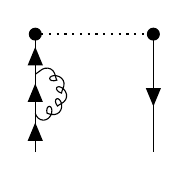
\begin{tikzpicture}[baseline=($(a)!0.5!(exa)$.base)]
			\begin{feynman}
				\node[dot] (a);
				\node[right=\FDWidth of a,dot] (b);
				\vertex[below=\FDHeight of a] (exa);
				\vertex[below=\FDHeight of b] (exb);
				\vertex at ($(exa)!0.33!(a)$) (a1);
				\vertex at ($(exa)!0.66!(a)$) (a2);
				\diagram*{
					(a) --[ghost] (b);
					(exa) --[fermion] (a1) --[fermion] (a2) --[fermion] (a);
					(b) --[fermion] (exb);
					(a1) --[gluon, half right,looseness=2] (a2);
				};
			\end{feynman}
		\end{tikzpicture}
		\caption{}
	\end{subfigure}
	\begin{subfigure}[b]{.49\linewidth}
		\centering
		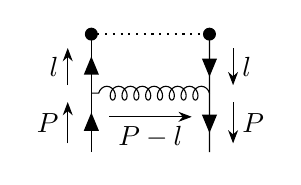
\begin{tikzpicture}[baseline=($(a)!0.5!(exa)$.base)]
			\begin{feynman}
				\node[dot] (a);
				\node[right=\FDWidth of a,dot] (b);
				\vertex[below=\FDHeight of a] (exa);
				\vertex[below=\FDHeight of b] (exb);
				\vertex at ($(exa)!0.5!(a)$) (a1);
				\vertex at ($(exb)!0.5!(b)$) (b1);
				\diagram*{
					(a) --[ghost] (b);
					(exa) --[fermion,momentum=\(P\)] (a1) --[fermion,momentum=\(l\)] (a);
					(b) --[fermion,momentum=\(l\)] (b1) --[fermion,momentum=\(P\)] (exb);
					(b1) --[gluon,rmomentum=\(P-l\)] (a1);
				};
			\end{feynman}
		\end{tikzpicture}
		\caption{}
		\label{1b}
	\end{subfigure}
	\caption{}
\end{figure}

The Feynman rule for the composite operator is
\begin{align}
	\feynmandiagram[small,baseline=(a.base),horizontal=a to b]{
		a[dot, label={\(p_1\),0}] --[ghost] b[dot, label={\(p_2\),z}];
	};=e^{-ip_2^zz} \gamma^z 
\end{align}
and two external lines give $\bar u(P)$ and $u(P)$ respectively. 

The first one is a quark self-energy correction
\begin{align}
	\bar u(P)e^{-iP^zz} \gamma^z \frac{i(\slashed{P}+m)}{P^2-m^2}\pqty{-i\Sigma_2(P)} u(P)
\end{align}
% where $\Sigma_2$ follows Peskin's result\cite{MichaelE.Peskin1995}. 

The second one is
\begin{align}
	&\bar u(P)\int\mmd[1]{l^0}\mmd[2]{\vb{l}_T}\eval{(-ig_st^a\gamma^{\mu})\frac{i(\slashed{l}+m)}{l^2-m^2}\gamma^z\frac{i(\slashed{l}+m)}{l^2-m^2}(-ig_st^a\gamma^{\nu})\tilde D_{G\mu\nu}^A(P-l)u(P)}_{l^z=xP^z}\notag\\
	&=-g_s^2C_F\bar u(P)\int\mmd[1]{l^0}\mmd[2]{\vb{l}_T}\eval{\gamma^{\mu}\frac{i(\slashed{l}+m)}{l^2-m^2}\gamma^z\frac{i(\slashed{l}+m)}{l^2-m^2}\gamma^{\nu}\tilde D_{G\mu\nu}^A(P-l)u(P)}_{l^z=xP^z}
\end{align}
For the definition of $\tilde D_{G\mu\nu}^A$, see Section~\ref{sec:conv}. There're in total 6 poles:
\begin{center}
	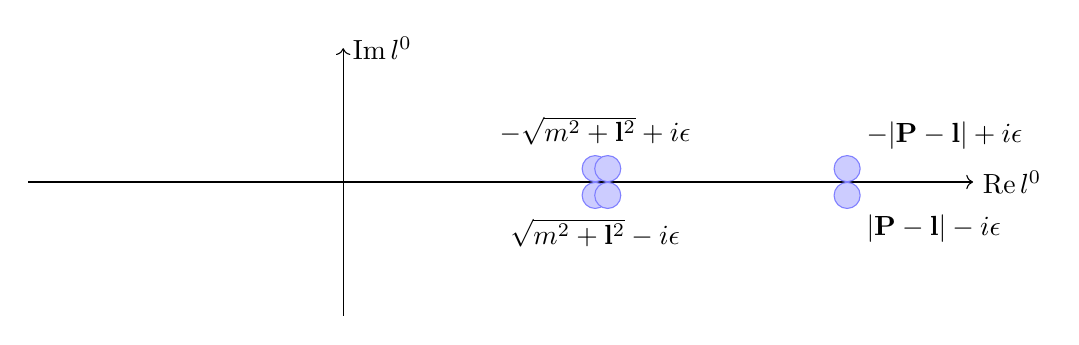
\begin{tikzpicture}[xscale=8,yscale=1.7]
		\draw[->] (-.5,0) -- (1,0) node[right]{$\Re l^0$};
		\draw[->] (0,-1) -- (0,1) node[right]{$\Im l^0$};
		\node at (.8,.1) [circle,draw=blue!50,fill=blue!20,label=above right:{$-\abs{\vb{P}-\vb{l}}+i\epsilon$}] {};
		\node at (.8,-.1) [circle,draw=blue!50,fill=blue!20,label=below right:{$\abs{\vb{P}-\vb{l}}-i\epsilon$}] {};
		\node at (0.4,.1) [circle,draw=blue!50,fill=blue!20,label=above:{$-\sqrt{m^2+\vb{l}^2}+i\epsilon$}] {};
		\node at (0.4,-.1) [circle,draw=blue!50,fill=blue!20,label=below:{$\sqrt{m^2+\vb{l}^2}-i\epsilon$}] {};
		\node at (0.42,.1) [circle,draw=blue!50,fill=blue!20] {};
		\node at (0.42,-.1) [circle,draw=blue!50,fill=blue!20] {};
	\end{tikzpicture}
\end{center}
For the result of numerator simplification, see Section~\ref{sec:dc1}
% The numerator is simplified as:
% \begin{align}
% 	&\bar u(P)\gamma^{\mu}(\slashed{P}-\slashed{l}+m)\gamma^z(\slashed{P}-\slashed{l}+m)\gamma^{\nu}u(P)\notag\\
% 	=&\left(2 l\cdot P-l^2-P^2+m^2\right) \bar u(P)\gamma^{\mu }\gamma^z\gamma^{\nu }u(P)+2 \left(l^z-P^z\right) \bar u(P)\gamma^{\mu }\slashed{l}\gamma^{\nu }u(P)\notag\\&-2 P^{\mu } \left(\bar u(P)\gamma^z\slashed{l}\gamma^{\nu }u(P)+\bar u(P)\slashed{l}\gamma^z\gamma^{\nu }u(P)-2	P^z \bar u(P)\gamma^{\nu }u(P)\right)
% \end{align}
% Adding the numerator of the axial gauge gluon propagator, the final result is 
% \begin{align}
% 	\frac{2 l^4 P^3}{\left(l^3\right)^2}+\frac{16 l^2 \left(P^3\right)^2}{l^3}-\frac{8 l^2 l^0P^0 P^3}{\left(l^3\right)^2}+4 l^2 P^3-\frac{4 l^2 l^0 P^0}{l^3}-8 m^2l^3+16 l^3 \left(P^3\right)^2-\frac{32 l^0 P^0 \left(P^3\right)^2}{l^3}\notag\\-8l^0 l^3 P^0+8 \left(l^3\right)^2 P^3-24 l^0 P^0 P^3+\frac{8\left(l^0\right)^2 \left(P^0\right)^2 P^3}{\left(l^3\right)^2}+\frac{8 \left(l^0\right)^2\left(P^0\right)^2}{l^3}+8 m^2 P^3+24 \left(P^3\right)^3
% \end{align}

\section{One Loop Quasi PDF (Feynman Gauge)}
In Feynman gauge, we must have the full definition of quasi PDF. For unpolarized quasi PDF
\begin{align}
	\tilde{q}(x)=\frac{1}{2} \int \frac{\dd z}{2 \pi} e^{i x P^{z} z}\langle P, S|\bar{\psi}(z) \gamma^z \exp \left[i g \mathcal{P} \int_{0}^{z} \dd z^{\prime} A^{a,z}\left(z^{\prime}\right) \mathrm{t}^{a}\right] \psi(0)| P, S\rangle
\end{align}
There're following 7 diagrams, 
\begin{figure}[!htpb]
	\centering
	\begin{subfigure}[b]{.24\linewidth}
		\centering
		\begin{tikzpicture}[baseline=($(a)!0.5!(exa)$.base)]
			\begin{feynman}
				\node[dot] (a);
				\node[right=\FDWidth of a,dot] (b);
				\vertex at ($(a)!0.5!(b)$) (o);
				\vertex[below=\FDHeight of a] (exa);
				\vertex[below=\FDHeight of b] (exb);
				\vertex at ($(exa)!0.5!(a)$) (a1);
				\vertex at ($(exb)!0.5!(b)$) (b1);
				\diagram*{
					(o) --[Eikonal] (b);
					(exa) --[fermion] (a1) --[fermion] (a);
					(b) --[fermion] (exb);
					(a1) --[gluon] (o);
				};
			\end{feynman}
		\end{tikzpicture}
		\caption{}
		\label{2a}
	\end{subfigure}
	\begin{subfigure}[b]{.24\linewidth}
		\centering
		\begin{tikzpicture}[baseline=($(a)!0.5!(exa)$.base)]
			\begin{feynman}
				\node[dot] (a);
				\node[right=\FDWidth of a,dot] (b);
				\vertex at ($(a)!0.5!(b)$) (o);
				\vertex[below=\FDHeight of a] (exa);
				\vertex[below=\FDHeight of b] (exb);
				\vertex at ($(exa)!0.5!(a)$) (a1);
				\vertex at ($(exb)!0.5!(b)$) (b1);
				\diagram*{
					(a) --[Eikonal] (o);
					(exa) --[fermion] (a);
					(b) --[fermion] (b1) --[fermion] (exb);
					(b1) --[gluon] (o);
				};
			\end{feynman}
		\end{tikzpicture}
		\caption{}
		\label{2b}
	\end{subfigure}
	\begin{subfigure}[b]{.24\linewidth}
		\centering
		\begin{tikzpicture}[baseline=($(a)!0.5!(exa)$.base)]
			\begin{feynman}
				\node[dot] (a);
				\node[right=\FDWidth of a,dot] (b);
				\vertex at ($(a)!0.3!(b)$) (o1);
				\vertex at ($(a)!0.7!(b)$) (o2);
				\vertex[below=\FDHeight of a] (exa);
				\vertex[below=\FDHeight of b] (exb);
				\diagram*{
					(a) --[Eikonal] (o1);
					(b) --[Eikonal] (o2);
					(exa) --[fermion] (a);
					(b) --[fermion] (exb);
					(o1) --[gluon, half right] (o2);
				};
			\end{feynman}
		\end{tikzpicture}
		\caption{}
		\label{2c}
	\end{subfigure}\\
	\begin{subfigure}[b]{.24\linewidth}
		\centering
		\begin{tikzpicture}[baseline=($(a)!0.5!(exa)$.base)]
			\begin{feynman}
				\node[dot] (a);
				\node[right=\FDWidth of a,dot] (b);
				\vertex at ($(a)!0.5!(b)$) (o);
				\vertex[below=\FDHeight of a] (exa);
				\vertex[below=\FDHeight of b] (exb);
				\vertex at ($(exa)!0.5!(a)$) (a1);
				\vertex at ($(exb)!0.5!(b)$) (b1);
				\diagram*{
					(o) --[Eikonal] (a);
					(exa) --[fermion] (a1) --[fermion] (a);
					(b) --[fermion] (exb);
					(a1) --[gluon] (o);
				};
			\end{feynman}
		\end{tikzpicture}
		\caption{}
		\label{2d}
	\end{subfigure}
	\begin{subfigure}[b]{.24\linewidth}
		\centering
		\begin{tikzpicture}[baseline=($(a)!0.5!(exa)$.base)]
			\begin{feynman}
				\node[dot] (a);
				\node[right=\FDWidth of a,dot] (b);
				\vertex at ($(a)!0.5!(b)$) (o);
				\vertex[below=\FDHeight of a] (exa);
				\vertex[below=\FDHeight of b] (exb);
				\vertex at ($(exa)!0.5!(a)$) (a1);
				\vertex at ($(exb)!0.5!(b)$) (b1);
				\diagram*{
					(b) --[Eikonal] (o);
					(exa) --[fermion] (a);
					(b) --[fermion] (b1) --[fermion] (exb);
					(b1) --[gluon] (o);
				};
			\end{feynman}
		\end{tikzpicture}
		\caption{}
		\label{2e}
	\end{subfigure}
	\begin{subfigure}[b]{.24\linewidth}
		\centering
		\begin{tikzpicture}[baseline=($(a)!0.5!(exa)$.base)]
			\begin{feynman}
				\node[dot] (a);
				\node[right=\FDWidth of a,dot] (b);
				\vertex at ($(a)!0.5!(b)$) (o);
				\vertex at ($(a)!0.2!(b)$) (o1);
				\vertex at ($(a)!0.8!(b)$) (o2);
				\vertex[below=\FDHeight of a] (exa);
				\vertex[below=\FDHeight of b] (exb);
				\diagram*{
					(a) --[Eikonal] (o);
					(exa) --[fermion] (a);
					(b) --[fermion] (exb);
					(o1) --[gluon, half right] (o);
				};
			\end{feynman}
		\end{tikzpicture}
		\caption{}
		\label{2f}
	\end{subfigure}
	\begin{subfigure}[b]{.24\linewidth}
		\centering
		\begin{tikzpicture}[baseline=($(a)!0.5!(exa)$.base)]
			\begin{feynman}
				\node[dot] (a);
				\node[right=\FDWidth of a,dot] (b);
				\vertex at ($(a)!0.5!(b)$) (o);
				\vertex at ($(a)!0.2!(b)$) (o1);
				\vertex at ($(a)!0.8!(b)$) (o2);
				\vertex[below=\FDHeight of a] (exa);
				\vertex[below=\FDHeight of b] (exb);
				\diagram*{
					(b) --[Eikonal] (o);
					(exa) --[fermion] (a);
					(b) --[fermion] (exb);
					(o) --[gluon, half right] (o2);
				};
			\end{feynman}
		\end{tikzpicture}
		\caption{}
		\label{2g}
	\end{subfigure}
	\caption{Diagrams of quasi PDF in Feynman gauge. }
\end{figure}

\appendix
\section{Conventions\label{sec:conv}}
The quark field $\psi$ reads
\begin{align}
	\psi(x)=\int \frac{\dd^{3} \vec{k}}{(2 \pi)^{3}} \frac{1}{2 E_{k}}\left[u(k) e^{-i k \cdot x} b_{k}+v(k)e^{ik\cdot x} d_{k}^{\dagger}\right]
\end{align}
and the projection of single particle state is 
\begin{align}
	\ket{p}=b_p^{\dagger}\ket{0}
\end{align}
\begin{align}
	\Bqty{b_{\vb{p}}^r,b_{\vb{q}}^{s\dagger}}=(2\pi)^32E\delta^{(3)}(\vb{p}-\vb{q})\delta^{rs}
\end{align}
The Dirac spinor is normalized to 
\begin{align}
	\bar u^s(p) u(p)=2m\delta^{rs}
\end{align}
With Gordon identity, one can derive\cite{Srednicki2007}
\begin{align}
	\bar u(P) \gamma^\mu u(P) =2P^\mu
\end{align}
The axial gauge propagator is 
\begin{align}
	\tilde D_G^{A\mu\nu}(p)=-i \delta_{a b}\left(g^{\mu \nu}-\frac{n^{\mu} p^{\nu}+n^{\nu} p^{\mu}}{n \cdot p}+n \cdot n \frac{p^{\mu} p^{\nu}}{(n \cdot p)^{2}}\right) \frac{1}{p^{2}}
\end{align} 
State contract with field:
\begin{align}
	\wick{\c{\psi}(x)\c{\ket{P}}}&=\int\mme{l}\frac{1}{2E_{\vb{l}}}\bqty{b_{\vb{l}}u(l)e^{-il\cdot x}+d_{\vb{l}}^{\dagger}v(l)e^{il\cdot x}}b_{\vb{P}}^{\dagger}\ket{0}\notag\\
	&=\int\mme{l}\frac{1}{2E_{\vb{l}}}u(l)e^{-il\cdot x}(2\pi)^32E\delta^{(3)}(\vb{l}-\vb{P})\ket{0}\notag\\
	&=u(P)e^{-iP\cdot x}
\end{align}
and correspondingly 
\begin{align}
	\wick{\c{\bra{P}}\c{\bar\psi}(x)}&=\bar u(P)e^{iP\cdot x}
\end{align}

\section{Wick Contraction\label{sec:Wick}}
\subsection{Axial Gauge}
Take diagram \ref{1b} as an example
\begin{center}
	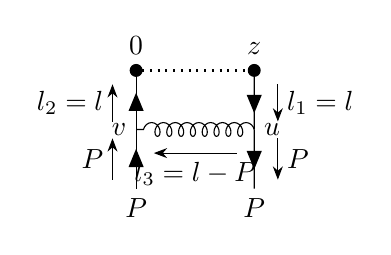
\begin{tikzpicture}[baseline=($(a)!0.5!(exa)$.base)]
		\begin{feynman}
			\node[dot, label=above:\(0\)] (a);
			\node[right=\FDWidth of a,dot, label=above:\(z\)] (b);
			\vertex[below=\FDHeight of a, label=below:\(P\)] (exa);
			\vertex[below=\FDHeight of b, label=below:\(P\)] (exb);
			\vertex[label=left:\(v\)] at ($(exa)!0.5!(a)$) (a1);
			\vertex[label=right:\(u\)] at ($(exb)!0.5!(b)$) (b1);
			\diagram*{
				(a) --[ghost] (b);
				(exa) --[fermion,momentum=\(P\)] (a1) --[fermion,momentum={\(l_2=l\)}] (a);
				(b) --[fermion,momentum={\(l_1=l\)}] (b1) --[fermion,momentum=\(P\)] (exb);
				(b1) --[gluon,momentum={\(l_3=l-P\)}] (a1);
			};
		\end{feynman}
	\end{tikzpicture}
\end{center}
This corresponds to 
\begin{align}
	&\frac{1}{4 \pi} \int \dd z e^{i x P^{z} z}\wick[offset=1.3em]{\langle \c1 P|\int\dd^4u\c1{\bar\psi}_u}\wick{\c1{\psi}_u \c2{A}_u\c1{\bar{\psi}}(z) \gamma^{z}\c3{\psi}(0)\int\dd^4v\c3{\bar\psi}_v\c4{\psi}_v \c2{A}_v| \c4 P\rangle}\\
	=&\frac{1}{4 \pi} \int \dd z e^{i x P^{z} z}\int\dd^4u\dd^4v\bar u(P)e^{iP\cdot u}\int\mm{l_1}\tilde D_F(l_1)e^{-il_1\cdot (u-z)}\gamma^z\int\mm{l_2}\tilde D_F(l_2)e^{-il_2\cdot (-v)}\notag\\&\int\mm{l_3}\tilde D_G(l_3)e^{-il_3\cdot (v-u)}u(P)e^{-iP\cdot v}\\
	=&\frac{1}{4 \pi} \int \dd z\int\dd^4u\dd^4v \int\mm{l_1}\int\mm{l_2}\int\mm{l_3}e^{i x P^{z} z+il_1\cdot z}e^{i(P-l_1+l_3)\cdot u}e^{i(l_2-l_3-P)\cdot v}\bar u(P)\tilde D_F(l_1)\gamma^z\tilde D_F(l_2)\notag\\&\tilde D_G(l_3)u(P)\\
	=&\frac{1}{4 \pi} \int \dd z \int\mm{l}e^{i x P^{z} z+il\cdot z}\bar u(P)\tilde D_F(l)\gamma^z\tilde D_F(l)\tilde D_G(l-P)u(P)\\
	=&\frac{1}{4 \pi} \int \dd z \int\mm{l}e^{i (x P^{z} -l^z) z}\bar u(P)\tilde D_F(l)\gamma^z\tilde D_F(l)\tilde D_G(l-P)u(P)\\
	=&\frac{1}{4 \pi} \int\mmd[1]{l^0}\int\mmd[2]{\vb{l}_T}\eval{\bar u(P)\tilde D_F(l)\gamma^z\tilde D_F(l)\tilde D_G(l-P)u(P)}_{l^z=xP^z}
\end{align}
where
\begin{align}
	\int \dd z e^{i (x P^{z} -l^z) z}=2\pi\delta(l^z-xP^z)
\end{align}
This indicates what the Feynman diagram actually means: a normal Feynman diagram with only 3-momentum integration, where the axial momentum is fixed by $l^z=xP^z$, and with an extra $1/4\pi$ factor. 

\subsection{Feynman Gauge}
Let's take diagram~\ref{2b} as an example:
\begin{center}
	\begin{tikzpicture}[baseline=($(a)!0.5!(exa)$.base)]
		\begin{feynman}
			\node[dot] (a);
			\node[right=\FDWidth of a,dot] (b);
			\vertex at ($(a)!0.5!(b)$) (o);
			\vertex[below=\FDHeight of a] (exa);
			\vertex[below=\FDHeight of b] (exb);
			\vertex at ($(exa)!0.5!(a)$) (a1);
			\vertex at ($(exb)!0.5!(b)$) (b1);
			\diagram*{
				(o) --[Eikonal,rmomentum=\(P-l\)] (b);
				(exa) --[fermion,momentum=\(P\)] (a);
				(b) --[fermion,momentum=\(l\)] (b1) --[fermion,momentum=\(P\)] (exb);
				(o) --[gluon,momentum'=\(P-l\)] (b1);
			};
		\end{feynman}
	\end{tikzpicture}
\end{center}
The one loop quasi PDF is
\begin{align}
	\tilde{q}^{(1)}_1(x)=\frac{1}{2} \int \frac{\dd z}{2 \pi} e^{i x P^{z} z}\langle P, S|\int\dd^4u\pqty{-ig_st^a}\bar\psi_u\psi_u A_u\bar{\psi}(z) \gamma^z \tilde{\mathcal{W}}[z, 0]  \psi(0)| P, S\rangle
\end{align}
where 
\begin{align}
	\tilde{\mathcal{W}}[z, 0] =\exp\left[i g_s \mathcal{P} \int_{0}^{z} \dd z^{\prime} A^{a,z}\left(z^{\prime}\right) \mathrm{t}^{a}\right]
\end{align}
We should rewrite the gauge link to the product of two gauge links connect to infinity
\begin{align}
	\tilde{\mathcal{W}}[z, 0] =\tilde{\mathcal{W}}[z, +\infty] \tilde{\mathcal{W}}[\infty, 0] 
\end{align}
and in one loop level it equals to 
\begin{align*}
	\exp\left[i g_s \mathcal{P} \int_{\infty}^{z} \dd z^{\prime} A^{a,z}\left(z^{\prime}\right) \mathrm{t}^{a}\right]\exp\left[i g_s \mathcal{P} \int_{0}^{\infty} \dd z^{\prime} A^{a,z}\left(z^{\prime}\right) \mathrm{t}^{a}\right]
	=\left[i g_s \mathcal{P} \int_{0}^{\infty} \dd z^{\prime} A^{a,z}\left(z^{\prime}\right) \mathrm{t}^{a}\right]-\left[i g_s \mathcal{P} \int_0^{\infty} \dd z^{\prime} A^{a,z}\left(z^{\prime}+z\right) \mathrm{t}^{a}\right]
\end{align*}
The path ordering gives
\begin{align}
	\mathcal{P} \int_{0}^{\infty} \dd z^{\prime} A^{a,z}\left(z^{\prime}\right) = \int \dd z^{\prime} A^{a,z}\left(z^{\prime}\right)\theta(z')=\int \dd z^{\prime} A^{a,z}\left(z^{\prime}\right)\int\frac{\dd w}{2\pi}\frac{ie^{-iwz' }}{w+i\epsilon}
\end{align}
and
\begin{align}
	\bqty{\mathcal{P} \int_{0}^{\infty} \dd z^{\prime} A^{a,z}\left(z^{\prime}\right)}^2 = \int \dd z^{\prime} A^{a,z}\left(z^{\prime}\right)\theta(z')\int \dd z^{\prime\prime} A^{a,z}\left(z^{\prime\prime}\right)\theta(z''-z')
\end{align}
with all momenta involved with $z'$ must be in the $z$-direction (the exponent is actually $z'n\cdot w$ if a four-vector $w$ actually exists). Consider the second gauge link first, the matrix element is then (discarding all couplings)
\begin{align*}
	&\langle P, S|\bar\psi_u\psi_u A_u\bar{\psi}(z) \gamma^z \int \dd z^{\prime} A^{a,z}\left(z^{\prime}+z\right) \int\frac{\dd w}{2\pi}\frac{ie^{-iwz' }}{w+i\epsilon}\psi(0)| P, S\rangle\\
	=&\int\dd^4u\langle P, S|\bar\psi_u\psi_u A_u\bar{\psi}(z) \gamma^z \int \dd z^{\prime} A^{a,z}\left(z^{\prime}+z\right) \psi(0)| P, S\rangle\int\frac{\dd w}{2\pi}\frac{ie^{-iwz' }}{w+i\epsilon}\\
	=&\int\dd^4u\wick{\c1{\langle P, S|}\c1{\bar\psi}_u\c2{\psi}_u \c3{A}_u\c2{\bar{\psi}}(z) \gamma^z \int \dd z^{\prime} \c3{A}^{a,z}\left(z^{\prime}+z\right) \c4{\psi}(0)\c4{| P, S\rangle}}\int\frac{\dd w}{2\pi}\frac{ie^{-iwz' }}{w+i\epsilon}\\
	=&\int \dd z^{\prime}\int\dd^4u \bar u(P)e^{iP\cdot u}\int\mm{l_1}\tilde D_F(l_1)e^{-il_1\cdot(u-z)}\int\mm{l_2}\tilde D_G(l_2)e^{-il_2\cdot(u-z'-z)}u(P)\int\frac{\dd w}{2\pi}\frac{ie^{-iwz' }}{w+i\epsilon}\\
	=&\int \dd z^{\prime}\int\dd^4u \int\mm{l_1}\int\mm{l_2}\int\frac{\dd w}{2\pi}\bar u(P)e^{i(P-l_1-l_2)\cdot u}e^{i(l_1+l_2)\cdot z}e^{-iwz' -il_2\cdot z'}\tilde D_F(l_1)\tilde D_G(l_2)u(P)\frac{i}{w+i\epsilon}\\
	=&\int \dd z^{\prime}\int\mm{l}\int\frac{\dd w}{2\pi}\bar u(P)e^{iP\cdot z}e^{-iwz' +i(P-l)^z z'}\tilde D_F(l)\tilde D_G(P-l)u(P)\frac{i}{w+i\epsilon}\\
	=&\bar u(P)e^{iP\cdot z}\int\mm{l}\tilde D_F(l)\tilde D_G(P-l)\frac{i}{P^z-l^z+i\epsilon}u(P)
\end{align*}
The complete quasi PDF at one loop is
\begin{align}
	&\frac{1}{2} \int \frac{\dd z}{2 \pi} e^{i x P^{z} z}\bar u(P)e^{iP\cdot z}\int\mm{l}\tilde D_F(l)\tilde D_G(P-l)\frac{i}{P^z-l^z+i\epsilon}u(P)\notag\\
	=&\frac{1}{2 P^z}\bar u(P)\int\mm{l}\tilde D_F(l)\tilde D_G(P-l)\frac{i}{P^z-l^z+i\epsilon}u(P)\delta(1-x)\notag
\end{align}
multiplied by those couplings. This basically established that the momentum of a gluon equals to the momentum of the eikonal line it attaches to. We then have the Feynman rule:
\begin{align}
	\feynmandiagram[small, horizontal=a to b,baseline=(a.base)]{
		a[dot] --[Eikonal,momentum=\(k\)] b;
	};=\frac{i}{n\cdot k+i\epsilon};\qquad
	\feynmandiagram[small, horizontal=a to b,baseline=(a.base)]{
		a --[Eikonal,rmomentum=\(k\)] b[dot];
	};=\frac{i}{n\cdot k+i\epsilon}
\end{align}
and for the gluon-eikonal vertex on the r.h.s., an extra minus sign is added for the normal $(ig_st^a)$.

The next job is to determine the Feynman rule for 
\begin{center}
	\begin{tikzpicture}[baseline=($(a)!0.5!(exa)$.base)]
		\begin{feynman}
			\node[dot] (a);
			\node[right=\FDWidth of a,dot] (b);
			\vertex at ($(a)!0.3!(b)$) (o1);
			\vertex at ($(a)!0.7!(b)$) (o2);
			\vertex[below=\FDHeight of a] (exa);
			\vertex[below=\FDHeight of b] (exb);
			\diagram*{
				(a) --[Eikonal,momentum=\(l\)] (o1);
				(b) --[Eikonal,momentum'=\(-l\)] (o2);
				(exa) --[fermion,momentum=\(P\)] (a);
				(b) --[fermion,momentum=\(P\)] (exb);
				(o1) --[gluon, half right,momentum'=\(l\)] (o2);
			};
		\end{feynman}
	\end{tikzpicture}\text{\qquad \&\qquad }
	\begin{tikzpicture}[baseline=($(a)!0.5!(exa)$.base)]
		\begin{feynman}
			\node[dot] (a);
			\node[right=\FDWidth of a,dot] (b);
			\vertex at ($(a)!0.5!(b)$) (o);
			\vertex at ($(a)!0.2!(b)$) (o1);
			\vertex at ($(a)!0.8!(b)$) (o2);
			\vertex[below=\FDHeight of a] (exa);
			\vertex[below=\FDHeight of b] (exb);
			\diagram*{
				(a) --[Eikonal,momentum=\(l\)] (o);
				(exa) --[fermion,momentum=\(P\)] (a);
				(b) --[fermion,momentum=\(P\)] (exb);
				(o1) --[gluon, half right,momentum'=\(l\)] (o);
			};
		\end{feynman}
	\end{tikzpicture}
\end{center}
The first one is
\begin{align}
	\frac{1}{2} \int \frac{\dd z}{2 \pi} e^{i x P^{z} z}\langle P, S|\bar{\psi}(z) \gamma^z \left[-i g_s \mathcal{P} \int_0^{\infty} \dd z^{\prime} A^{a,z}\left(z^{\prime}+z\right) \mathrm{t}^{a}\right]\left[i g_s \mathcal{P} \int_{0}^{\infty} \dd z^{\prime} A^{a,z}\left(z^{\prime}\right) \mathrm{t}^{a}\right]  \psi(0)| P, S\rangle
\end{align}
Let's look at the coupling-free form:
\begin{align*}
	&\int \frac{\dd z}{2 \pi} e^{i x P^{z} z}\langle P, S|\bar{\psi}(z) \gamma^z \left[ \mathcal{P} \int_0^{\infty} \dd z^{\prime} A^{a,z}\left(z^{\prime}+z\right) \right]\left[ \mathcal{P} \int_{0}^{\infty} \dd z^{\prime\prime} A^{a,z}\left(z^{\prime\prime}\right) \right]  \psi(0)| P, S\rangle\\
	=&\int \frac{\dd z}{2 \pi} e^{i x P^{z} z}\langle P, S|\bar{\psi}(z) \gamma^z
	\int \dd z^{\prime} A^{a,z}\left(z^{\prime}+z\right)
	\int \dd z^{\prime\prime} A^{a,z}\left(z^{\prime\prime}\right)  \psi(0)| P, S\rangle\int\frac{\dd w}{2\pi}\frac{ie^{-iwz' }}{w+i\epsilon}\int\frac{\dd h}{2\pi}\frac{ie^{-ihz'' }}{h+i\epsilon}\\
	=&\int \frac{\dd z}{2 \pi} e^{i x P^{z} z}\wick{\langle \c1P, S|\c1{\bar{\psi}}(z) \gamma^z
	\int \dd z^{\prime} \c2A^{a,z}\left(z^{\prime}+z\right)
	\int \dd z^{\prime\prime} \c2A^{a,z}\left(z^{\prime\prime}\right)  \c1\psi(0)| \c1P, S\rangle}\int\frac{\dd w}{2\pi}\frac{ie^{-iwz' }}{w+i\epsilon}\int\frac{\dd h}{2\pi}\frac{ie^{-ihz'' }}{h+i\epsilon}\\
	=&\int \frac{\dd z}{2 \pi} e^{i x P^{z} z}\bar u(P)e^{iP\cdot z}\gamma^z\int\dd z'\dd z''\int\mm{l}\tilde D_G(l)e^{-il\cdot(z''-z'-z)}u(P)\int\frac{\dd w}{2\pi}\frac{ie^{-iwz' }}{w+i\epsilon}\int\frac{\dd h}{2\pi}\frac{ie^{-ihz'' }}{h+i\epsilon}\\
	=&\bar u(P)\int \frac{\dd z}{2 \pi} e^{i (x-1) P^{z} z+il^zz}\gamma^z\int\dd z'\dd z''\int\mm{l}\tilde D_G(l)\int\frac{\dd w}{2\pi}\frac{i}{w+i\epsilon}\int\frac{\dd h}{2\pi}\frac{i}{h+i\epsilon}e^{-i(w-l)\cdot z'}e^{-i(l+h)\cdot z''} u(P)\\
	=&\bar u(P)\int \frac{\dd z}{2 \pi} e^{-i (1-x) P^{z} z+il^zz}\gamma^z\int\mm{l}\tilde D_G(l)\frac{i}{l^z+i\epsilon}\frac{i}{-l^z+i\epsilon} u(P)\\
	=&\bar u(P)\gamma^z\int\mm{l}\tilde D_G(l)\frac{i}{l^z+i\epsilon}\frac{i}{-l^z+i\epsilon}\delta(l^z-(1-x)P^z) u(P)\\
\end{align*}
The second one is 
\begin{align}
	\frac{1}{2} \int \frac{\dd z}{2 \pi} e^{i x P^{z} z}\langle P, S|\bar{\psi}(z) \gamma^z \frac{\left[i g_s \mathcal{P} \int_{0}^{\infty} \dd z^{\prime} A^{a,z}\left(z^{\prime}\right) \mathrm{t}^{a}\right]\left[i g_s \mathcal{P} \int_{0}^{\infty} \dd z^{\prime\prime} A^{a,z}\left(z^{\prime\prime}\right) \mathrm{t}^{a}\right]}{2}  \psi(0)| P, S\rangle
\end{align}
The coupling-free form is 
\begin{align*}
	&\int \frac{\dd z}{2 \pi} e^{i x P^{z} z}\langle P, S|\bar{\psi}(z) \gamma^z \left[ \mathcal{P} \int_{0}^{\infty} \dd z^{\prime} A^{a,z}\left(z^{\prime}\right) \right]\left[ \mathcal{P} \int_{0}^{\infty} \dd z^{\prime\prime} A^{a,z}\left(z^{\prime\prime}\right) \right]  \psi(0)| P, S\rangle\\
	=&\int \frac{\dd z}{2 \pi} e^{i x P^{z} z}\langle P, S|\bar{\psi}(z) \gamma^z \int \dd z^{\prime} A^{a,z}\left(z^{\prime}\right)\int \dd z^{\prime\prime} A^{a,z}\left(z^{\prime\prime}\right)  \psi(0)| P, S\rangle\int\frac{\dd w}{2\pi}\frac{ie^{-iwz' }}{w+i\epsilon}\int\frac{\dd h}{2\pi}\frac{ie^{-ih(z''-z') }}{h+i\epsilon}\\
	=&\int \frac{\dd z}{2 \pi} e^{i x P^{z} z}\wick{\langle \c1P, S|\c1{\bar{\psi}}(z) \gamma^z \int \dd z^{\prime} \c2A^{a,z}\left(z^{\prime}\right)\int \dd z^{\prime\prime} \c2A^{a,z}\left(z^{\prime\prime}\right)  \c1\psi(0)| \c1P, S\rangle}
	\int\frac{\dd w}{2\pi}\frac{ie^{-iwz' }}{w+i\epsilon}\int\frac{\dd h}{2\pi}\frac{ie^{-ih(z''-z') }}{h+i\epsilon}\\
	=&\int \frac{\dd z}{2 \pi} e^{i x P^{z} z}\bar u(P)e^{iP\cdot z} \gamma^z \int \dd z^{\prime} \int \dd z^{\prime\prime} \int\mm{l}\tilde D_G(l)e^{-il\cdot(z''-z')}  u(P)
	\int\frac{\dd w}{2\pi}\frac{ie^{-iwz' }}{w+i\epsilon}\int\frac{\dd h}{2\pi}\frac{ie^{-ih(z''-z') }}{h+i\epsilon}\\
	=&\bar u(P)\int \frac{\dd z}{2 \pi} e^{-i (1-x) P^{z} z+il^zz} \gamma^z \int \dd z^{\prime} \int \dd z^{\prime\prime} \int\mm{l}\tilde D_G(l) 
	\int\frac{\dd w}{2\pi}\frac{i}{w+i\epsilon}\int\frac{\dd h}{2\pi}\frac{i}{h+i\epsilon}e^{-i(w-l-h)\cdot z'}e^{-i(h+l)\cdot z''} u(P)\\
	=&\bar u(P) \gamma^z \int\mm{l}\tilde D_G(l) 
	\frac{i}{0+i\epsilon}\frac{i}{-l^z+i\epsilon} \delta(l^z-(1-x)P^z)u(P)
\end{align*}
Diagram~\ref{2g} is 
\begin{align}
	\frac{1}{2} \int \frac{\dd z}{2 \pi} e^{i x P^{z} z}\langle P, S|\bar{\psi}(z) \gamma^z \frac{\left[-i g_s \mathcal{P} \int_{0}^{\infty} \dd z^{\prime} A^{a,z}\left(z^{\prime}+z\right) \mathrm{t}^{a}\right]\left[- i g_s \mathcal{P} \int_{0}^{\infty} \dd z^{\prime\prime} A^{a,z}\left(z^{\prime\prime}+z\right) \mathrm{t}^{a}\right]}{2}  \psi(0)| P, S\rangle
\end{align}
and it behaves exactly like \ref{2f}, since those extra $(+z)$s will be cancelled in the Wick contraction. 


\section{Diagram~\ref{1b} Comparing\label{sec:dc1}}
Let's start with
\begin{align}
	&\bar u(P)\int\mmd[1]{l^0}\mmd[2]{\vb{l}_T}\eval{(-ig_st^a\gamma^{\mu})\frac{i(\slashed{l}+m)}{l^2-m^2}\gamma^z\frac{i(\slashed{l}+m)}{l^2-m^2}(-ig_st^a\gamma^{\nu})\tilde D_{G\mu\nu}^A(P-l)u(P)}_{l^z=xP^z}\notag\\
	=&-g_s^2C_F\bar u(P)\int\mmd[1]{l^0}\mmd[2]{\vb{l}_T}\eval{\gamma^{\mu}\frac{i(\slashed{l}+m)}{l^2-m^2}\gamma^z\frac{i(\slashed{l}+m)}{l^2-m^2}\gamma^{\nu}\tilde D_{G\mu\nu}^A(P-l)u(P)}_{l^z=xP^z}\notag\\
	=&-ig_s^2C_F\bar u(P)\int\mmd[1]{l^0}\mmd[2]{\vb{l}_T}\gamma^{\mu}\frac{\slashed{l}+m}{l^2-m^2}\gamma^z\frac{\slashed{l}+m}{l^2-m^2}\gamma^{\nu}\frac{1}{(P-l)^2}u(P)\notag\\&\eval{\bqty{\bar{g}^{\mu \nu }-\frac{n^{\nu } \left(P^{\mu }-l^{\mu }\right)+n^{\mu} \left(P^{\nu }-l^{\nu }\right)}{n\cdot (P-l)}+\frac{n^2 \left(P^{\mu }-l^{\mu }\right) \left(P^{\nu }-l^{\nu }\right)}{\left(n\cdot P-n\cdot l\right)^2}}}_{l^z=xP^z}
\end{align}
We consider the numerator as a first step
\begin{align}
	\bar u(P)\gamma^{\mu}(\slashed{l}+m)\gamma^z(\slashed{l}+m)\gamma^{\nu}\bqty{\pqty{P-l}^2\tilde D_{G\mu\nu}^A(P-l)}u(P)
\end{align}
We can separate the gluon propagator into there parts. The first one gives a metric tensor and the final result 
\begin{align}
	4 l^3 \left(m \bar{u}(P) u(P)-\bar{u}(P) \slashed{l} u(P)\right)-2 \left(m^2-l^2\right) \bar{u}(P) \gamma^3 u(P)
\end{align}

The combined result can be further separated with respect to the structure of gamma matrices. The first one is for $\bar u(P)\slashed{l}u(P)$: 
\begin{align*}
	&\frac{2 l^z \left(2 l^z \left(P^z-l^z\right)-l^2+m^2\right)}{\left(l^2-m^2\right)^2 (P-l)^2\left(l^z-P^z\right)^2}\\
	=&-\frac{4 \pqty{l^z}^2  }{\left(l^2-m^2\right)^2 (P-l)^2\left(l^z-P^z\right)}-\frac{2 l^z }{\left(l^2-m^2\right) (P-l)^2\left(l^z-P^z\right)^2}\\
\end{align*}
for $\bar u(P)u(p)$:
\begin{align*}
	&\frac{2 m l^z \left(-6 l^z P^z+4 \left(l^z\right)^2+2 \left(P^z\right)^2+l^2-m^2\right)}{\left(l^2-m^2\right)^2(l-P)^2 \left(l^z-P^z\right)^2}\\
	=&\frac{2 m l^z \left(-4 l^z P^z+4 \left(l^z\right)^2\right)}{\left(l^2-m^2\right)^2(l-P)^2 \left(l^z-P^z\right)^2}
	+\frac{2 m l^z \left(-2 l^z P^z+2 \left(P^z\right)^2\right)}{\left(l^2-m^2\right)^2(l-P)^2 \left(l^z-P^z\right)^2}
	+\frac{2 m l^z \left(l^2-m^2\right)}{\left(l^2-m^2\right)^2(l-P)^2 \left(l^z-P^z\right)^2}\\
	=&\frac{8 m \left(l^z\right)^2 \left( l^z-  P^z\right)}{\left(l^2-m^2\right)^2(l-P)^2 \left(l^z-P^z\right)^2}
	-\frac{4 m l^z P^z\left( l^z - P^z\right)}{\left(l^2-m^2\right)^2(l-P)^2 \left(l^z-P^z\right)^2}
	+\frac{2 m l^z \left(l^2-m^2\right)}{\left(l^2-m^2\right)^2(l-P)^2 \left(l^z-P^z\right)^2}\\
	=&\frac{8 m \left(l^z\right)^2 }{\left(l^2-m^2\right)^2(l-P)^2 \left(l^z-P^z\right)}
	-\frac{4 m l^z P^z}{\left(l^2-m^2\right)^2(l-P)^2 \left(l^z-P^z\right)}
	+\frac{2 m l^z }{\left(l^2-m^2\right)(l-P)^2 \left(l^z-P^z\right)^2}\\
	=&\frac{4 m \left(l^z\right)^2 }{\left(l^2-m^2\right)^2(l-P)^2 \left(l^z-P^z\right)}
	+\frac{4 m \left(l^z\right)^2-4 m l^z P^z}{\left(l^2-m^2\right)^2(l-P)^2 \left(l^z-P^z\right)}
	+\frac{2 m l^z }{\left(l^2-m^2\right)(l-P)^2 \left(l^z-P^z\right)^2}\\
	=&\frac{4 m \left(l^z\right)^2 }{\left(l^2-m^2\right)^2(l-P)^2 \left(l^z-P^z\right)}
	+\frac{4 m l^z\left(l^z-  P^z\right)}{\left(l^2-m^2\right)^2(l-P)^2 \left(l^z-P^z\right)}
	+\frac{2 m l^z }{\left(l^2-m^2\right)(l-P)^2 \left(l^z-P^z\right)^2}\\
	=&\frac{4 m \left(l^z\right)^2 }{\left(l^2-m^2\right)^2(l-P)^2 \left(l^z-P^z\right)}
	+\frac{4 m l^z}{\left(l^2-m^2\right)^2(l-P)^2 }
	+\frac{2 m l^z }{\left(l^2-m^2\right)(l-P)^2 \left(l^z-P^z\right)^2}
\end{align*}
for $\bar u(P)\gamma^zu(p)$:
\begin{align*}
	&\frac{(l-P)^2 \left(2 l^z \left(P^z-l^z\right)-l^2+m^2\right)+2 \left(m^2-l^2\right) P^z \left(l^z-P^z\right)}{\left(l^2-m^2\right)^2(l-P)^2 \left(l^z-P^z\right)^2}\\
	=&\frac{(l-P)^2 \left(2 l^z \left(P^z-l^z\right)-l^2+m^2\right)}{\left(l^2-m^2\right)^2(l-P)^2 \left(l^z-P^z\right)^2}
	+\frac{2 \left(m^2-l^2\right) P^z \left(l^z-P^z\right)}{\left(l^2-m^2\right)^2(l-P)^2 \left(l^z-P^z\right)^2}\\
	=&\frac{ 2 l^z \left(P^z-l^z\right)-l^2+m^2}{\left(l^2-m^2\right)^2 \left(l^z-P^z\right)^2}
	-\frac{2  P^z }{\left(l^2-m^2\right)(l-P)^2 \left(l^z-P^z\right)}\\
	=&\frac{ 2 l^z \left(P^z-l^z\right)}{\left(l^2-m^2\right)^2 \left(l^z-P^z\right)^2}
	-\frac{l^2-m^2}{\left(l^2-m^2\right)^2 \left(l^z-P^z\right)^2}
	-\frac{2  P^z }{\left(l^2-m^2\right)(l-P)^2 \left(l^z-P^z\right)}\\
	=&-\frac{ 2 l^z }{\left(l^2-m^2\right)^2 \left(l^z-P^z\right)}
	-\frac{1}{\left(l^2-m^2\right) \left(l^z-P^z\right)^2}
	-\frac{2  P^z }{\left(l^2-m^2\right)(l-P)^2 \left(l^z-P^z\right)}\\
\end{align*}
The total result is
\begin{align}
	&\begin{aligned}
		\bar u(P)
		\Bqty{&-\frac{4 \pqty{l^z}^2 \slashed{l} }{\left(l^2-m^2\right)^2 (l-P)^2\left(l^z-P^z\right)}
		-\frac{2 l^z \slashed{l}}{\left(l^2-m^2\right) (l-P)^2\left(l^z-P^z\right)^2}\\&
		+\frac{4 m \left(l^z\right)^2 }{\left(l^2-m^2\right)^2(l-P)^2 \left(l^z-P^z\right)}
		+\frac{4 m l^z}{\left(l^2-m^2\right)^2(l-P)^2 }
		+\frac{2 m l^z }{\left(l^2-m^2\right)(l-P)^2 \left(l^z-P^z\right)^2}\\&
		-\frac{ 2 l^z \gamma^z}{\left(l^2-m^2\right)^2 \left(l^z-P^z\right)}
		-\frac{\gamma^z}{\left(l^2-m^2\right) \left(l^z-P^z\right)^2}
		-\frac{2  P^z \gamma^z}{\left(l^2-m^2\right)(l-P)^2 \left(l^z-P^z\right)}
			}
		u(P)
	\end{aligned}\\
	\phantom{=}&
	\begin{aligned}
		=\bar u(P)
		\Bqty{&\frac{-4  \left(l^z\right)^2\pqty{\slashed{l}-m} }{\left(l^2-m^2\right)^2 (l-P)^2\left(l^z-P^z\right)}
		-\frac{2 l^z \pqty{\slashed{l}-m } }{\left(l^2-m^2\right) (l-P)^2\left(l^z-P^z\right)^2}
		+\frac{4 m l^z}{\left(l^2-m^2\right)^2(l-P)^2 }\\&
		-\frac{ 2 l^z \gamma^z}{\left(l^2-m^2\right)^2 \left(l^z-P^z\right)}
		-\frac{\gamma^z}{\left(l^2-m^2\right) \left(l^z-P^z\right)^2}
		-\frac{2  P^z \gamma^z}{\left(l^2-m^2\right)(l-P)^2 \left(l^z-P^z\right)}
			}
		u(P)
	\end{aligned}\\
	\phantom{=}&
	\begin{aligned}
		=\bar u(P)
		\Bqty{&\frac{-4  \left(l^z\right)^2\pqty{\slashed{l}-m} +4 m l^z\left(l^z-P^z\right)}{\left(l^2-m^2\right)^2 (l-P)^2\left(l^z-P^z\right)}
		-\frac{2 l^z \pqty{\slashed{l}-m } +2  P^z \gamma^z\left(l^z-P^z\right)}{\left(l^2-m^2\right) (l-P)^2\left(l^z-P^z\right)^2}\\&
		-\frac{ 2 l^z \gamma^z}{\left(l^2-m^2\right)^2 \left(l^z-P^z\right)}
		-\frac{\gamma^z}{\left(l^2-m^2\right) \left(l^z-P^z\right)^2}
			}
		u(P)
	\end{aligned}\\
	\phantom{=}&
	\begin{aligned}
		=\bar u(P)
		\Bqty{&-\frac{4  \left(l^z\right)^2\pqty{\slashed{l}-2m}+4ml^zP^z }{\left(l^2-m^2\right)^2 (l-P)^2\left(l^z-P^z\right)}
		-\frac{2 l^z \pqty{\slashed{l}-m +P^z\gamma^z} -2  \pqty{P^z}^2 \gamma^z}{\left(l^2-m^2\right) (l-P)^2\left(l^z-P^z\right)^2}\\&
		-\frac{ 2 l^z \gamma^z}{\left(l^2-m^2\right)^2 \left(l^z-P^z\right)}
		-\frac{\gamma^z}{\left(l^2-m^2\right) \left(l^z-P^z\right)^2}
			}
		u(P)
	\end{aligned}
\end{align}

Xiong's result is 
\begin{align}
	&-i g_{s}^{2} C_{F} \int \frac{d^{4} k}{(2 \pi)^{4}} \bar{u}(P)\left[
		\frac{2 \gamma^{z}}{\left(k^{2}-m^{2}\right)(P-k)^{2}}
		+\frac{4\left(2 m-k^{z}\right) \not k}{\left(k^{2}-m^{2}\right)^{2}(P-k)^{2}}\right.\notag\\ 
		&\left.+\frac{2\left(k^{z} \gamma^{z}+\not k-m\right)}{\left(k^{2}-m^{2}\right)(P-k)^{2}\left(P^{z}-k^{z}\right)}
		-\frac{\gamma^{z}}{(P-k)^{2}\left(P^{z}-k^{z}\right)^{2}}
		\right] P^{z} \delta\left(k^{z}-x P^{z}\right) u(P)
\end{align}
As we discussed earlier, it can be dissected into
\begin{align}
	&\frac{4\left(2 m-k^{z}\right) \slashed k}{\left(k^{2}-m^{2}\right)^{2}(P-k)^{2}}+\frac{2\slashed k}{\left(k^{2}-m^{2}\right)(P-k)^{2}\left(P^{z}-k^{z}\right)} &\bar u(P)\slashed{k}u(P)\\
	&\frac{-2m}{\left(k^{2}-m^{2}\right)(P-k)^{2}\left(P^{z}-k^{z}\right)} &\bar u(P)u(P)\\
	&\frac{2 \gamma^z}{\left(k^{2}-m^{2}\right)(P-k)^{2}}+\frac{2k^{z} \gamma^{z}}{\left(k^{2}-m^{2}\right)(P-k)^{2}\left(P^{z}-k^{z}\right)}-\frac{\gamma^{z}}{(P-k)^{2}\left(P^{z}-k^{z}\right)^{2}} &\bar u(P)\gamma^zu(P)
\end{align}

\bibliography{../Bib}
\bibliographystyle{apsrev4-1}
\end{document}
